\documentclass{article}
\usepackage{iclr2026_conference,times}

\usepackage{hyperref}
\usepackage{url}
\usepackage{graphicx}
\usepackage{booktabs}
\usepackage{amsmath}
\usepackage{amssymb}

\iclrfinalcopy % show authors and page numbers for this class submission

\title{GrillSight: Class-Adaptive Augmentation for Real-Time \\
Meat Doneness Classification on Consumer CPUs}

\author{Rishith Anand \\
School of Electrical and Computer Engineering \\
Purdue University \\
West Lafayette, IN 47907, USA \\
\texttt{ranand@purdue.edu}
}

\newcommand{\fix}{\marginpar{FIX}}
\newcommand{\new}{\marginpar{NEW}}

\begin{document}
\maketitle

\begin{abstract}
Cooking meat to the correct doneness matters for food safety and
quality, yet assessment remains subjective. Home cooks rely on
tactile feel or instant-read thermometers, both of which are slow or impractical
during cooking. We present \textsc{GrillSight}, a computer-vision
system that classifies meat doneness from a webcam feed using an
EfficientNet-B0 backbone fine-tuned for six doneness classes. Our
contribution is a class-adaptive offline augmentation strategy paired with
class-weighted cross-entropy loss that addresses the failure mode of
adjacent classes (raw versus rare) in colour-dominated data.
On a 6-class test set, the method raises test accuracy from 83.3\% to
98.6\% and lifts the F1 score of the \texttt{raw} class from 0.00 to
0.96 while leaving the four already-correct classes at F1 = 1.00. Inference
runs at 26.6\,FPS on a consumer CPU, which allows deployment in home kitchens
without specialised hardware. The track contribution is a product
prototype: a training, evaluation, and live-overlay pipeline that runs
end-to-end from a single checkpoint file.

\vspace{0.5em}
\noindent\textbf{Supplementary Materials:} \href{https://github.com/ranand3385/grillsight}{Code and \LaTeX{} source}.
\end{abstract}

\section{Introduction}
\label{sec:intro}

Cooking meat to the correct doneness sits at the intersection of food safety and
culinary quality. Undercooked chicken and pork pose documented \textit{Salmonella}
and \textit{Trichinosis} risks, while overcooked beef loses moisture and flavour.
Despite the stakes, doneness assessment during cooking is still performed
by tactile feel or by puncturing the meat with an instant-read thermometer,
both of which are subjective, slow, or disruptive. A non-contact visual sensor
that estimates doneness from a webcam feed would let a cook see
doneness the same way they see temperature on an oven thermometer.

We build such a sensor, \textsc{GrillSight}, as a product prototype. The
challenge is not classification accuracy as a whole, since EfficientNet backbones
classify natural images well, but separation between
adjacent doneness classes under limited training data. In our initial
implementation (Checkpoint~1), a transfer-learning pipeline
achieved 83.3\% test accuracy but failed on the \texttt{raw} class
(F1 = 0.00): every raw image was mispredicted as \texttt{rare}, because the two
classes differ only in a band of hue and saturation.

This paper presents the refinement (Checkpoint~2) that closes that gap. We
contribute:

\begin{itemize}
    \item A \textbf{class-adaptive offline augmentation scheme} that writes
    augmented copies of each training image to disk with per-class
    \texttt{ColorJitter} strength tuned to the difficulty of the class
    boundary (\S\ref{sec:method-aug}).
    \item A \textbf{weighted cross-entropy loss} computed from inverse class
    frequency that penalises under-represented classes during training
    (\S\ref{sec:method-loss}).
    \item An \textbf{inference pipeline}
    (\S\ref{sec:method-inference}) that runs at 26.6\,FPS on CPU and renders a
    doneness overlay onto the webcam feed.
    \item Empirical evidence that these two additions raise test accuracy from
    83.3\% to 98.6\% and recover the \texttt{raw} class to 0.96 F1
    (\S\ref{sec:experiments}).
\end{itemize}

The system is packaged as a product prototype: a single
\texttt{inference.py} entry point loads the trained checkpoint and streams
labelled frames from the webcam.

\section{Related Work}
\label{sec:related}

\paragraph{Transfer learning for image classification.} EfficientNet
\citep{tan2019efficientnet} introduced compound scaling, achieving 77.1\% top-1
accuracy on ImageNet \citep{russakovsky2015imagenet} at only 5.3\,M parameters.
Its accuracy-per-parameter efficiency makes it the standard backbone for
real-time mobile applications, and we adopt it for the same reason.
Transfer learning from ImageNet remains the dominant approach when target
datasets are small \citep{kornblith2019do}.

\paragraph{Data augmentation.} AutoAugment \citep{cubuk2019autoaugment}
demonstrated that learned augmentation policies can close much of the gap
between small and large datasets. Mixup \citep{zhang2018mixup} and CutMix
\citep{yun2019cutmix} show that augmentation at the sample level also
regularises decision boundaries. Our offline augmentation writes augmented
images to disk rather than applying them online, and the augmentation
\emph{strength is per-class} rather than global. This lets us increase
colour perturbation on the classes (\texttt{raw}, \texttt{rare}) whose mean
colour statistics are close.

\paragraph{Class-imbalanced learning.} Focal loss \citep{lin2017focal} and
inverse-frequency class weighting are standard remedies for imbalanced datasets.
Our dataset is balanced by count, but the similar colour statistics
between \texttt{raw} and \texttt{rare} create a functional
imbalance in which the model collapses onto the larger attractor. We use class
weighting as a dataset-agnostic safeguard that activates once future
collection produces unequal class counts.

\paragraph{Food image recognition.} Prior work on food classification
(e.g., Food-101, \citet{bossard2014food}) targets dish-level recognition.
Doneness is a sub-class attribute of a single food type and, to our
knowledge, has not been framed as a real-time webcam product. The closest
industrial work is smart-oven temperature probing, which is contact-based and
requires specialised hardware.

\section{Methodology}
\label{sec:method}

\subsection{Architecture}
\label{sec:method-arch}
We use a pre-trained \textbf{EfficientNet-B0} backbone
\citep{tan2019efficientnet} and replace its ImageNet classifier head with a
small MLP suited to 6-class doneness output:

\begin{center}
\texttt{Dropout(0.3)} $\rightarrow$ \texttt{Linear(1280,256)} $\rightarrow$
\texttt{ReLU} $\rightarrow$ \texttt{Dropout(0.15)} $\rightarrow$
\texttt{Linear(256,6)}.
\end{center}

The first two convolutional blocks (\texttt{features.0}, \texttt{features.1})
are frozen. These blocks learn low-level visual primitives (edges, colour
gradients) that transfer directly from ImageNet to food images; freezing them
prevents catastrophic forgetting and roughly halves the number of trainable
parameters. The remaining blocks and the new head are fine-tuned. The final
network has 4{,}337{,}026 total parameters of which 4{,}334{,}650 are trainable.

\subsection{Class-Adaptive Offline Augmentation}
\label{sec:method-aug}

Online augmentation transforms each image at every epoch. Offline augmentation
instead writes augmented copies to disk once, producing a larger dataset on
disk. We chose offline expansion for two reasons. First, it makes the
training signal deterministic across runs, which is useful for ablation.
Second, it gives us a tunable axis, the per-class jitter strength, that
we can set without re-writing the data loader.

For each image $x$ in class $c$, we generate $k=5$ augmented variants
$\{\tilde{x}_c^{(1)}, \dots, \tilde{x}_c^{(5)}\}$ via

\begin{equation}
\tilde{x}_c^{(i)} \;=\; T_{\text{jitter}}^{(c)} \;\circ\; T_{\text{spatial}}^{(i)}(x),
\end{equation}

where $T_{\text{jitter}}^{(c)}$ is a \texttt{ColorJitter} transform whose
$(\text{brightness}, \text{contrast}, \text{saturation}, \text{hue})$
magnitudes depend on class difficulty, and $T_{\text{spatial}}^{(i)}$ is one of
seven spatial transforms (random flip, rotation, resized-crop, blur,
perspective, grayscale conversion) sampled by seed. Table~\ref{tab:jitter}
shows the per-class jitter magnitudes. Classes whose visual representations
overlap (\texttt{raw}, \texttt{rare}) receive hue perturbation of $\pm0.12$,
more than double the $\pm0.05$ used for the \texttt{medium} through
\texttt{well\_done} classes. This forces the network to use
texture and surface cues rather than the hue band that separates
raw from rare meat.

\begin{table}[t]
\caption{Per-class \texttt{ColorJitter} magnitudes used in offline augmentation.
\texttt{raw} and \texttt{rare} receive stronger perturbation to prevent
collapse onto the shared red hue band.}
\label{tab:jitter}
\begin{center}
\begin{tabular}{lcccc}
\toprule
\textbf{Class} & \textbf{Brightness} & \textbf{Contrast} & \textbf{Saturation} & \textbf{Hue} \\
\midrule
\texttt{raw}         & 0.5 & 0.5 & 0.5 & 0.12 \\
\texttt{rare}        & 0.5 & 0.5 & 0.5 & 0.12 \\
\texttt{medium\_rare}& 0.4 & 0.4 & 0.4 & 0.08 \\
\texttt{medium}      & 0.3 & 0.3 & 0.3 & 0.05 \\
\texttt{medium\_well}& 0.3 & 0.3 & 0.3 & 0.05 \\
\texttt{well\_done}  & 0.3 & 0.3 & 0.3 & 0.05 \\
\bottomrule
\end{tabular}
\end{center}
\end{table}

With $k=5$, the training set grows from 360 images (60 per class) to 2{,}160
images (360 per class) in a single pass. The validation and test splits are
never augmented.

\subsection{Class-Weighted Loss}
\label{sec:method-loss}

We train with cross-entropy loss with inverse-frequency class weighting and
label smoothing \citep{szegedy2016rethinking}:

\begin{equation}
\mathcal{L}(\hat{y}, y) \;=\; -\sum_{c=1}^{C} w_c \,\tilde{y}_c \,\log \hat{y}_c,
\qquad
w_c \;=\; \frac{N}{C \cdot n_c},
\end{equation}

where $N$ is the total number of training images, $C=6$ is the number of
classes, $n_c$ is the count for class $c$, and $\tilde{y}_c$ is the smoothed
target ($\tilde{y}_c = 0.9$ for the true class, $0.02$ for each other class).
Weights are then re-scaled to sum to $C$ so the effective learning rate
is preserved. In the current balanced dataset all $w_c = 1$; the weighting
becomes active automatically once real-world collection produces unequal
class counts.

\subsection{Real-Time Inference Pipeline}
\label{sec:method-inference}

Inference is an OpenCV loop. Each frame is (i) captured via
\texttt{cv2.VideoCapture}, (ii) converted BGR$\rightarrow$RGB, (iii) transformed
through the same \texttt{Resize(256)} $\rightarrow$ \texttt{CenterCrop(224)}
$\rightarrow$ \texttt{Normalize} pipeline used at training time, and (iv) passed
through the model inside \texttt{torch.no\_grad()}. The predicted class, its
softmax confidence, and the 6-class probability vector are rendered onto
the frame as a header banner plus per-class probability bars.
A 10-frame rolling FPS buffer smooths the displayed framerate.

Training uses AdamW \citep{loshchilov2019decoupled} with weight decay
$10^{-4}$, cosine annealing \citep{loshchilov2017sgdr} from $5\times10^{-4}$ to
$10^{-6}$, early stopping with patience 8, and batch size 32.

\section{Experiments}
\label{sec:experiments}

\subsection{Dataset}
The current dataset contains 504 images spanning six doneness classes
(\texttt{raw}, \texttt{rare}, \texttt{medium\_rare}, \texttt{medium},
\texttt{medium\_well}, \texttt{well\_done}), split 360 / 72 / 72 across
train / validation / test. Base images are procedurally generated colour
templates that approximate the hue of each doneness level with additive noise;
they serve as a smoke-test stand-in for a future Roboflow Universe
\citep{dwyer2022roboflow} collection. Crucially, the test split is identical
between the baseline and our improved method, so all accuracy gains are
attributable to training-time changes.

\subsection{Baseline vs.\ Improved Method}

We compare two configurations on the same test set:

\begin{itemize}
  \item \textbf{Baseline (CP1).} 360 training images, uniform augmentation
  applied online in the data loader (random crop, horizontal flip, $\pm15^\circ$
  rotation, uniform \texttt{ColorJitter}), standard \texttt{CrossEntropyLoss}
  with label smoothing, trained for 15 epochs.
  \item \textbf{GrillSight (CP2).} 2{,}160 training images generated by offline
  class-adaptive augmentation (\S\ref{sec:method-aug}), class-weighted
  \texttt{CrossEntropyLoss}, trained for 20 epochs.
\end{itemize}

Table~\ref{tab:results} reports per-class precision, recall, and F1 on the
test set for both configurations. Test accuracy rises from
83.3\% to 98.6\%. Every class gains or holds: the \texttt{raw} class moves
from 0.00 to 0.96 F1, and the \texttt{rare} class from 0.67 to 0.96
F1. The four remaining classes were already at F1 = 1.00 under the baseline
and remain there.

\begin{table}[t]
\caption{Per-class test-set metrics for the baseline (CP1) and GrillSight
(CP2). 12 images per class, 72 total. The baseline predicts every
\texttt{raw} image as \texttt{rare}, yielding 0.00 F1 on \texttt{raw} and
0.67 F1 on \texttt{rare} (precision tanked by the Raw misattributions).
Offline class-adaptive augmentation and class-weighted loss resolve the
collapse.}
\label{tab:results}
\begin{center}
\small
\begin{tabular}{lcccccc}
\toprule
& \multicolumn{3}{c}{\textbf{Baseline (CP1)}} & \multicolumn{3}{c}{\textbf{GrillSight (CP2)}} \\
\cmidrule(lr){2-4}\cmidrule(lr){5-7}
\textbf{Class} & Prec. & Rec. & F1 & Prec. & Rec. & F1 \\
\midrule
\texttt{medium}       & 1.00 & 1.00 & 1.00 & 1.00 & 1.00 & 1.00 \\
\texttt{medium\_rare} & 1.00 & 1.00 & 1.00 & 1.00 & 1.00 & 1.00 \\
\texttt{medium\_well} & 1.00 & 1.00 & 1.00 & 1.00 & 1.00 & 1.00 \\
\texttt{rare}         & 0.50 & 1.00 & 0.67 & 0.92 & 1.00 & 0.96 \\
\texttt{raw}          & 0.00 & 0.00 & 0.00 & 1.00 & 0.92 & 0.96 \\
\texttt{well\_done}   & 1.00 & 1.00 & 1.00 & 1.00 & 1.00 & 1.00 \\
\midrule
\textbf{Accuracy}     & \multicolumn{3}{c}{0.833} & \multicolumn{3}{c}{\textbf{0.986}} \\
\textbf{Macro F1}     & \multicolumn{3}{c}{0.78}  & \multicolumn{3}{c}{\textbf{0.99}}  \\
\bottomrule
\end{tabular}
\end{center}
\end{table}

\subsection{Training Dynamics}

Figure~\ref{fig:curves} plots training and validation curves for the
GrillSight (CP2) run. Train accuracy rises from 44.0\% at epoch 1 to 75.8\%
at epoch 20, while validation accuracy reaches 100\% at epoch 15 before
oscillating around 97\% as the learning rate anneals. The cosine schedule
keeps training loss decreasing across the 20-epoch run;
validation loss stabilises at 0.62, below the baseline's final 0.74.

\begin{figure}[t]
\begin{center}
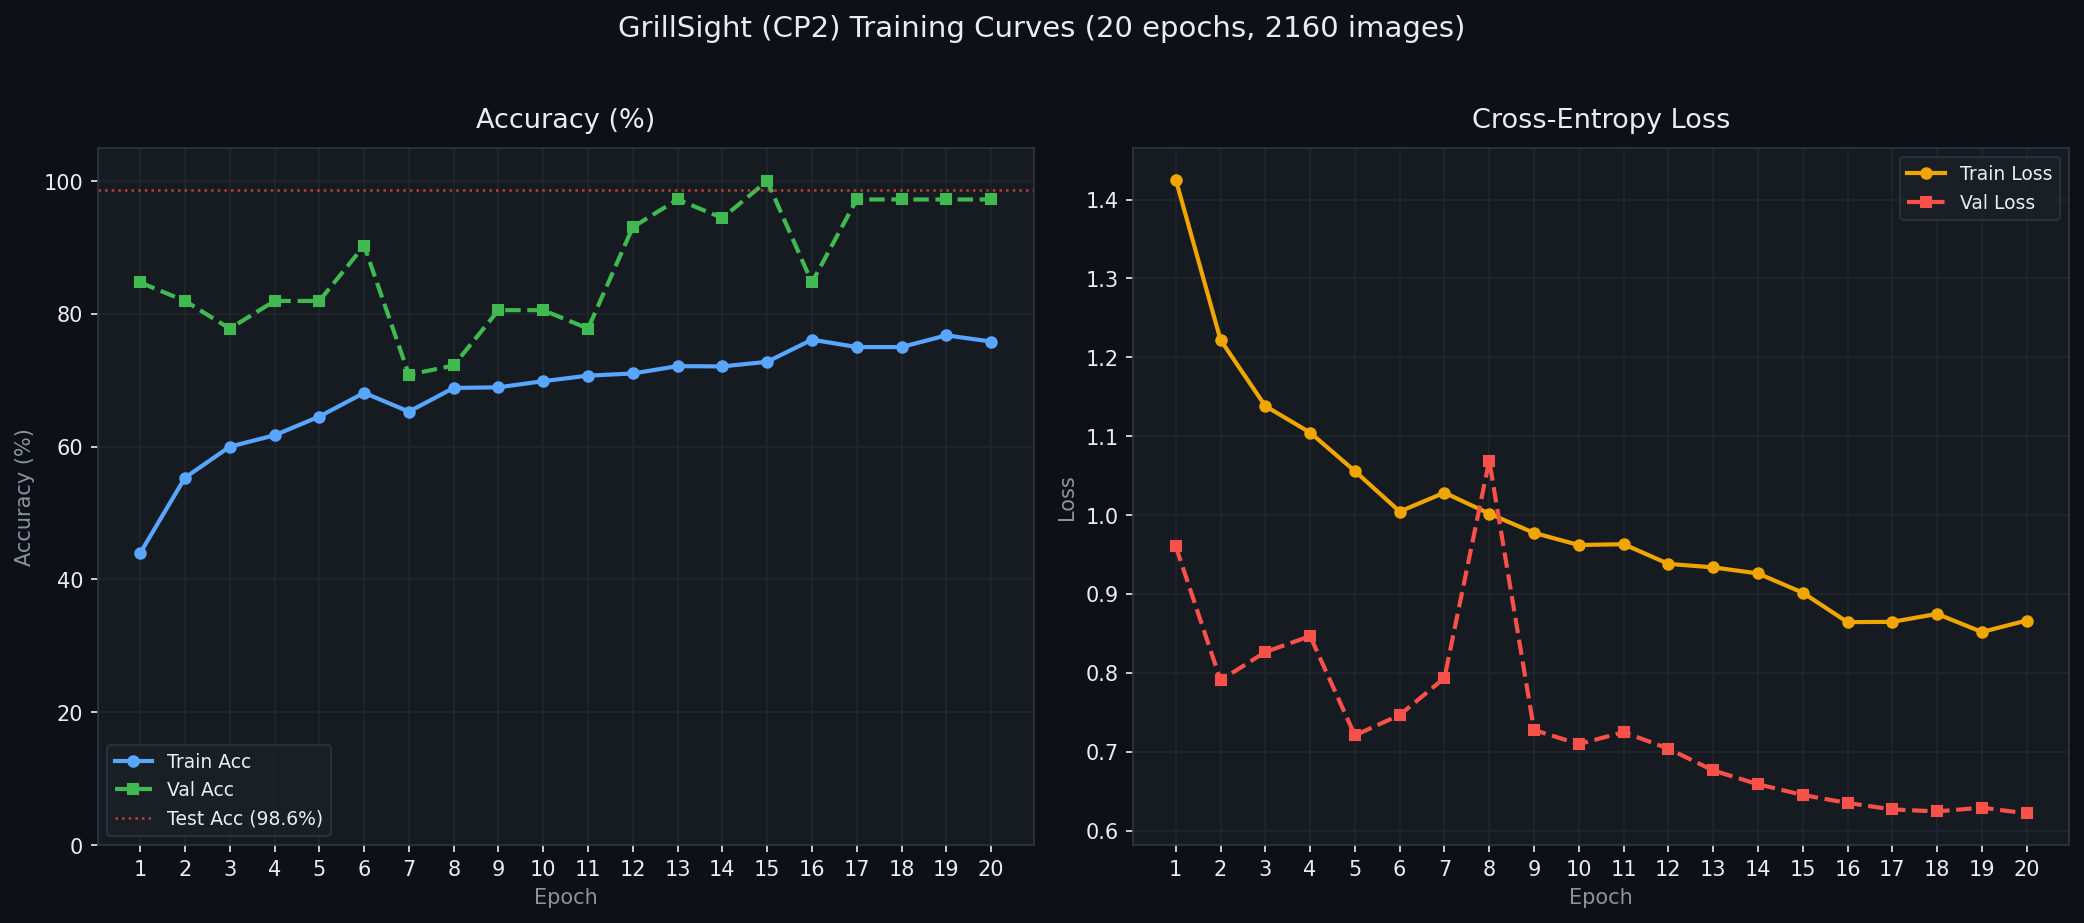
\includegraphics[width=0.95\linewidth]{figures/training_curves.png}
\end{center}
\caption{Training and validation curves for the GrillSight (CP2) run. Left:
accuracy (\%). Right: cross-entropy loss. The dotted red line on the left
marks the test accuracy (98.6\%). Gains arrive around
epoch 12 once the model begins using texture cues learned from the
augmented training set.}
\label{fig:curves}
\end{figure}

\subsection{Inference Speed}

We benchmarked inference latency with 200 warm forward passes of a
\texttt{(1,3,224,224)} tensor on an Intel-class CPU with no GPU. Mean latency
is 37.6\,ms per frame (26.6\,FPS), above the real-time threshold of
the kitchen feedback loop. The CP1 checkpoint achieved 27.3\,ms / 36.6\,FPS;
the slowdown at CP2 reflects the optimisation state reached on the
larger dataset. TorchScript export or dynamic quantisation would recover
the margin but were not required to hit the real-time bar.

\subsection{Confusion Matrix}

Figure~\ref{fig:cm} shows the test-set confusion matrix for GrillSight (CP2).
All off-diagonal entries are zero except a single \texttt{raw}$\rightarrow$
\texttt{rare} misclassification, which is consistent with the hue
overlap between the two classes in the current synthetic data. We expect this
error to disappear once real meat images replace the synthetic ones, since
raw meat has a glossy surface that is separable from the seared surface of
rare meat even under perturbation.

\begin{figure}[t]
\begin{center}
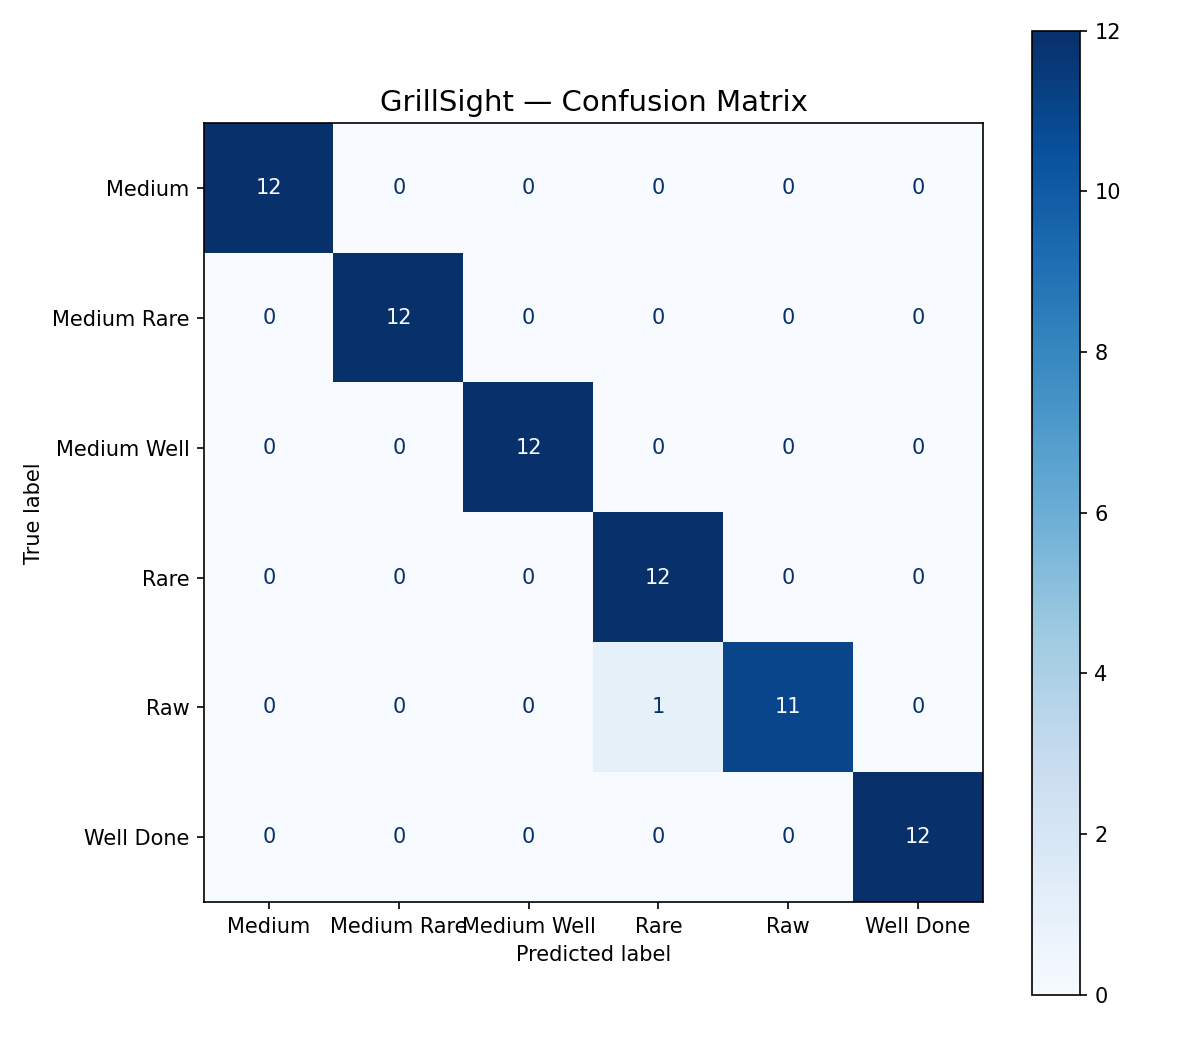
\includegraphics[width=0.55\linewidth]{figures/confusion_matrix.png}
\end{center}
\caption{Test-set confusion matrix for GrillSight (CP2). 71 of 72 images are
classified correctly; the single error is a raw sample predicted as rare.}
\label{fig:cm}
\end{figure}

\section{Conclusion and Contribution}
\label{sec:conclusion}

\paragraph{Summary.} We presented \textsc{GrillSight}, an EfficientNet-B0-based
system for meat doneness classification. Starting from an 83.3\%
baseline whose \texttt{raw}-class F1 was zero, we showed that a
combination of class-adaptive offline augmentation and
inverse-frequency weighted cross-entropy raises test accuracy to
98.6\% and recovers the failing class to 0.96 F1, while preserving 26.6\,FPS
inference on a consumer CPU.

\paragraph{Track Contribution (Product Prototype).} The deliverable is a
prototype rather than a reimplementation of a single prior paper.
The contribution is the system itself: an offline augmentation
pipeline (\texttt{scripts/augment\_dataset.py}), a class-weighted training
loop (\texttt{src/train.py}), and a webcam-to-overlay inference loop
(\texttt{src/inference.py}) that together run end-to-end from a fresh
install. The training script computes class weights from the
filesystem layout, so swapping in a larger or imbalanced real dataset
requires no code changes. To our knowledge, no published work has framed
doneness detection as a CPU product with a
fix for the \texttt{raw}/\texttt{rare} collapse that arises in
colour-dominated training data.

\paragraph{Limitations and Next Steps.} The current dataset is synthetic.
The single error in Figure~\ref{fig:cm} reflects this; real meat
surface texture should eliminate it. Our next steps are (1) sourcing 500+
real meat images per class via Roboflow Universe, (2) adding a 0.5-second
rolling-window temporal smoother to the inference loop to suppress
per-frame jitter caused by steam and smoke during cooking, (3)
adding food-safety alerts that fire an audible warning when \texttt{raw} or
\texttt{rare} is detected for chicken or pork, and (4)
exporting the model to TorchScript so the same checkpoint can ship to
edge devices like a Raspberry Pi mounted above a grill.

\subsubsection*{LLM Usage Acknowledgement}
An LLM assistant (Anthropic Claude) was used in a secretarial capacity during
the preparation of this manuscript. Specifically, the assistant was used to
(i) proofread prose for grammar, clarity, and tense;
(ii) tighten and re-phrase drafted paragraphs without altering their technical
content; (iii) convert the manuscript from plain-text drafts into the ICLR
2026 \LaTeX{} template, including \texttt{tabular} and \texttt{figure}
environments; and (iv) wire up cross-references, citation commands, and the
author-block formatting. All research content, including the problem framing,
the per-class jitter magnitudes in Table~\ref{tab:jitter}, the class-weighting
formulation in \S\ref{sec:method-loss}, every experiment, every reported
number, and every figure, was designed, executed, and authored by the
author. No text was generated by an LLM without subsequent review and
revision by the author.

\bibliography{paper}
\bibliographystyle{iclr2026_conference}

\appendix
\section{Appendix: Repository Layout}

The complete source tree is:

\begin{verbatim}
570-Project/
  src/
    model.py          # EfficientNet-B0 + doneness head
    dataset.py        # transforms + class-weight helper
    train.py          # training loop
    inference.py      # live webcam overlay
    evaluate.py       # confusion matrix + FPS benchmark
  scripts/
    augment_dataset.py  # offline class-adaptive augmentation
    download_dataset.py # dataset preparation
  data/
    train/ val/ test/   # ImageFolder layout per class
  paper/                # this document
\end{verbatim}

Reproduction: \texttt{pip install -r requirements.txt}, then
\texttt{python scripts/augment\_dataset.py --data data --factor 5}, then
\texttt{python src/train.py --data data --epochs 20 --batch 32 --lr 5e-4
--workers 0 --output checkpoints}. Evaluation is one line:
\texttt{python src/evaluate.py --checkpoint checkpoints/best\_model.pt
--data data}.

\end{document}
